%%%%%%%%%%%%%%%%%%%%%%%%%%%%%%%%%%%%%%%%%%%%%%%%%%%%%%%%%%%%%%%%%%%%%%%%%%%%%%%%
%2345678901234567890123456789012345678901234567890123456789012345678901234567890
%        1         2         3         4         5         6         7         8

\documentclass[a4, 10 pt, conference]{ieeeconf}  % Comment this line out if you need a4paper

%\documentclass[a4paper, 10pt, conference]{ieeeconf}      % Use this line for a4 paper

\IEEEoverridecommandlockouts                              % This command is only needed if 
                                                          % you want to use the \thanks command

\overrideIEEEmargins                                      % Needed to meet printer requirements.

% See the \addtolength command later in the file to balance the column lengths
% on the last page of the document

% The following packages can be found on http:\\www.ctan.org
%\usepackage{graphics} % for pdf, bitmapped graphics files
%\usepackage{epsfig} % for postscript graphics files
%\usepackage{mathptmx} % assumes new font selection scheme installed
%\usepackage{times} % assumes new font selection scheme installed
%\usepackage{amsmath} % assumes amsmath package installed
%\usepackage{amssymb}  % assumes amsmath package installed
\usepackage{multicol}
\usepackage{tcolorbox}
\usepackage{cuted,tcolorbox,lipsum}
\usepackage{xcolor}
\usepackage{pgfplots}
\usepackage{textcomp}
\usepackage{siunitx}


\title{\LARGE \bf
Introduction to Machine Learning (SS 2023)\\ Programming Project
\vspace{-3em}
}


%\author{Someone Anyone$^{1}$ and Xiang Zhang$^{2}$% <-this % stops a space
%}


\begin{document}


\maketitle
\vspace{-3em}
\thispagestyle{empty}
\pagestyle{empty}

\begin{strip}
\begin{tcolorbox}[
size=tight,
colback=white,
boxrule=0.2mm,
left=3mm,right=3mm, top=3mm, bottom=1mm
%width=\dimexpr\linewidth1cm\relax % Hier die Breite anpassen
]
{\begin{multicols}{3}% replace 3 with 2 for 2 authors.

\textbf{Author 1}       \\
Last name:	Erhart            \\  % Enter first name
First name:	Jonas           \\  % Enter first name
Matrikel Nr.: 	11906977             \\  % Enter Matrikel number

\columnbreak

\textbf{Author 2}       \\ 
Last name:	Untermann            \\  % Enter first name
First name:	Sven          \\  % Enter first name
Matrikel Nr.:	11906555           \\  % Enter Matrikel number

\columnbreak

% only four three person team
% \textbf{Author 3}       \\
% Last name:              \\  % Enter first name
% First name:             \\  % Enter first name
% Matrikel Nr.:               \\  % Enter Matrikel number

\end{multicols}}
\end{tcolorbox}
\end{strip}

%%%%%%%%%%%%%%%%%%%%%%%%%%%%%%%%%%%%%%%%%%%%%%%%%%%%%%%%%%%%%%%%%%%%%%%%%%%%%%%%


%{\color{blue}
 % \noindent This template outlines the sections that your report must 
  %contain. Inside each section, we provide pointers to what you should
 % write about in that section (in blue text).  \linebreak

%\noindent \textbf{Please remove all the text in blue in your report!
 % Your report should be 2 pages for regular teams (excluding references!)
  %and 3 pages for the three person team.}  }

\section{Introduction}
\label{sec:intro}

{\color{black}

\begin{itemize}
	\textbfn The ability to identify fraudulent transactions is of great interest to the payments industry. In this project, we will utilize a binary classifier trained on a transactions dataset to detect fraud. The dataset consists of various features related to the transactions, along with the amount of each transaction. Our objective is to determine, based on these features, whether a transaction is fraudulent or not. The dataset contains 227,845 instances of transactions with 29 different features. Throughout this project, we will train and evaluate the classifier using these data
\end{itemize}
}


\section{Implementation / ML Process}
\label{sec:methods}

{\color{black}

\begin{itemize} 
	%\item 
	\textbfn The given dataset consists of transaction data with a binary classification task of identifying fraud transactions. Before selecting a model, it is important to analyze the data and address any issues, such as class imbalance.\newline

	\textbfn The dataset is highly imbalanced, with a majority of legitimate transactions (Class 0) and a minority of fraud transactions (Class 1). To balance the dataset, the "Class 1" samples can be oversampled using the resample function from scikit-learn. This creates a new dataset with an equal number of samples for both classes. The balanced dataset is then used for training the models.\newline

	\textbfn After balancing the dataset, we can proceed with selecting a suitable model. The script provides options for different algorithms, including Logistic Regression, Decision Trees, Random Forests, Multilayer Perceptron (Neural Network), and AdaBoost. Each algorithm is defined with its corresponding hyperparameter search space.\\

	\textbfn The chosen algorithm family for this problem is ensemble methods, which includes Decision Trees, Random Forests, and AdaBoost. Ensemble methods combine multiple weak models to create a stronger model with improved generalization and robustness. These algorithms are suitable for this problem because they can handle complex relationships in the data and have the ability to learn from imbalanced datasets.\\

	\textbfnIt Is important to note that the provided script does not cover the entire data preprocessing and feature engineering pipeline. It assumes that the data is already preprocessed and ready for model training. In a real-world scenario, additional steps such as data cleaning, feature scaling, and feature selection may be required before training the models. 
\end{itemize}
}

\section{Results}
\label{sec:results}

{\color{Black}

\begin{itemize}
\documentclass{\newline}
\textbfIn The diagram compares the accuracy of different models, including Logistic Regression, Decision Tree, Random Forest, Neural Network, and AdaBoost. The accuracy metric measures how well the models are able to make correct predictions. The diagram shows that the Random Forest model achieves the highest accuracy, followed by the Decision Tree and AdaBoost. Logistic Regression and Neural Network models have slightly lower accuracy values. These differences in accuracy could be attributed to factors such as the complexity of the models, data quality, or chosen hyperparameters. The accuracy diagram provides an overview of model performance in terms of accuracy and helps in selecting the best model for the task at hand.\end{itemize}
%\begin{document}
\begin{figure}[h]
  \centering
  % Accuracy-Diagramm
  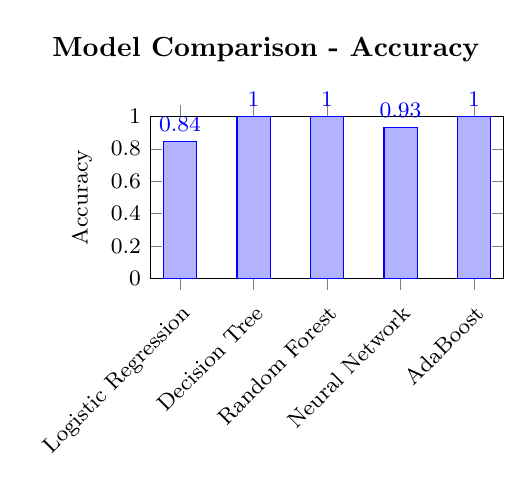
\begin{tikzpicture}
    \begin{axis}[
        ybar,
        width=0.5\textwidth,
        height=0.3\textwidth,
        ylabel=Accuracy,
        symbolic x coords={Logistic Regression, Decision Tree, Random Forest, Neural Network, AdaBoost},
        xtick=data,
        xticklabel style={rotate=45, anchor=north east}, % Schrift auf x-Achse schräg
        nodes near coords,
        nodes near coords align={vertical},
        ymin=0, ymax=1,
        bar width=12pt,
        font=\footnotesize % Manuell Schriftgröße anpassen
      ]
      \addplot coordinates {
        (Logistic Regression,0.8437)
        (Decision Tree,0.9989)
        (Random Forest,1.0000)
        (Neural Network,0.9331)
        (AdaBoost,1.0000)
        
      };
    \end{axis}
    \node at (current bounding box.north) [above=1ex, font=\bfseries] {Model Comparison - Accuracy};
  \end{tikzpicture}
  \caption{Accuracy-Diagramms} \newline
  \end{figure} 
  \begin{itemize}
  \textbfn The second diagram, the ROC (Receiver Operating Characteristic) curves of the models are shown. The ROC curve evaluates the trade-off between the true positive rate (TPR) and the false positive rate (FPR) for different classification thresholds. It provides a visual representation of the models' ability to distinguish between positive and negative classes.

Comparing the ROC curves, we observe that the Random Forest model achieves the highest AUC (Area Under the Curve), indicating its superior performance in distinguishing between legitimate and fraudulent transactions. The Decision Tree and AdaBoost models also exhibit high AUC values. However, the Logistic Regression and Neural Network models show slightly lower AUC values.

The differences in the ROC curves highlight the variations in sensitivity to false positives and true positives among the models. A higher ROC AUC score indicates better overall classification performance. :
\end{itemize}


%The Accuracy diagram (Figure 1) compares the accuracy of the different models. It shows that the Random Forest model has the highest accuracy of 100\%, followed by the Decision Tree model with 99.89\%.
  
 
\begin{figure}[h]
\centering
  % ROC-Diagramm
  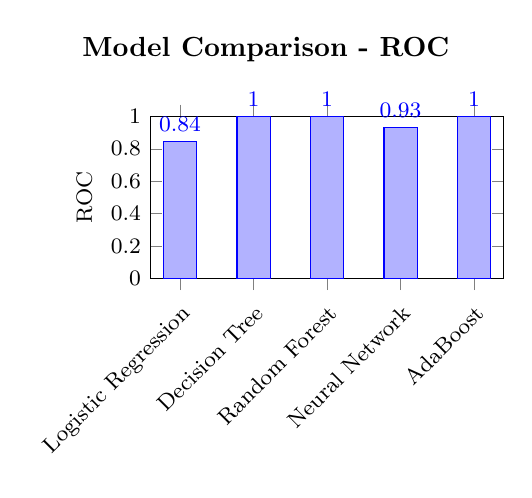
\begin{tikzpicture}
    \begin{axis}[
        ybar,
        width=0.5\textwidth,
        height=0.3\textwidth,
        ylabel=ROC,
        symbolic x coords={Logistic Regression, Decision Tree, Random Forest, Neural Network, AdaBoost},
        xtick=data,
        xticklabel style={rotate=45, anchor=north east}, % Schrift auf x-Achse schräg
        nodes near coords,
        nodes near coords align={vertical},
        ymin=0, ymax=1,
        bar width=12pt,
        font=\footnotesize % Manuell Schriftgröße anpassen
      ]
      \addplot coordinates {
        (Logistic Regression,0.8437)
        (Decision Tree,0.9989)
        (Random Forest,1.0000)
        (Neural Network,0.9331)
        (AdaBoost,1.0000)
      };
    \end{axis}
    \node at (current bounding box.north) [above=1ex, font=\bfseries] {Model Comparison - ROC};
  \end{tikzpicture}
  \caption{ROC-Diagramms} 
  \end{figure}
  \begin{itemize}
  \textbfIn In the third diagram, the Sensitivity/Specificity scores of the models are presented. Sensitivity (TPR) measures the ability of the model to correctly identify fraudulent transactions, while Specificity (TNR) represents its ability to correctly identify legitimate transactions.

Comparing the scores, we observe that the Random Forest and AdaBoost models achieve the highest scores for both TPR and TNR. The Decision Tree model also demonstrates high scores for TPR and TNR. However, the Logistic Regression and Neural Network models exhibit slightly lower scores, indicating a relatively lower ability to accurately classify both fraudulent and legitimate transactions.

These differences in Sensitivity/Specificity scores highlight the variations in the models' performance in accurately classifying instances. Models with higher scores for both TPR and TNR generally exhibit better discrimination between fraudulent and legitimate transactions. :
%The ROC diagram (Figure 2) compares the ROC curve of the different models. It shows that all models have a very high AUC (Area Under the Curve), with the Random Forest model achieving the best performance with an AUC of 1.0. 
\end{itemize}



\begin{figure}[h]
%\centering
\hspace*{0cm}
\begin{minipage}[b]{0.8\textwidth}
  % Sensitivity/Specificity-Diagramm
  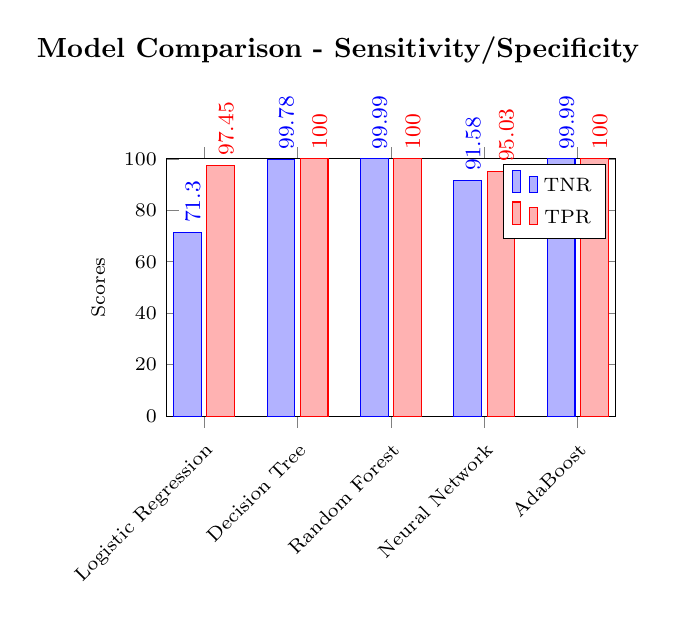
\begin{tikzpicture}
    \begin{axis}[
        ybar,
        width=0.6\textwidth,
        height=0.4\textwidth,
        ylabel=Scores,
        symbolic x coords={Logistic Regression, Decision Tree, Random Forest, Neural Network, AdaBoost},
        xtick=data,
        xticklabel style={rotate=45, anchor=north east},
        nodes near coords,
        nodes near coords align={vertical},
        nodes near coords style={
          font=\footnotesize,
          rotate=90,
          anchor=west,
          yshift=-2pt
          },
        ymin=0, ymax=100,
        bar width=10pt,
        font=\scriptsize
      ]
      \addplot coordinates {
        (Logistic Regression,71.30)
        (Decision Tree,99.78)
        (Random Forest,99.99)
        (Neural Network,91.58)
        (AdaBoost,99.99)
      };
      \addplot coordinates {
        (Logistic Regression,97.45)
        (Decision Tree,100.00)
        (Random Forest,100.00)
        (Neural Network,95.03)
        (AdaBoost,100.00)
      };
      \legend{TNR, TPR}
    \end{axis}
    \node at (current bounding box.north) [above=1ex, font=\bfseries] {Model Comparison - Sensitivity/Specificity};
  \end{tikzpicture}

\end{minipage}
\caption{Sensitivity/Specificity-Diagramm}
%\end {center}
\end{figure}


%\end{document}
}

\section{Discussion}
\label{sec:discuss}
\sisetup{output-decimal-marker={\textasciitilde}}
{\color{black}
\begin{itemize}
	\textbfn 
	The performance of our model (\(\sim\)\num{95}\% roc auc score on unseen data) is attributed to the AdaBoost algorithm which uses Boosting to train 	weak learners. This in combination with some data preprocessing is very effective for developing a decision tree classifier using our 			imbalanced dataset. 
	The idea of using an ensemble algorithm to extend a classifier arose when a test using a decision tree classifier lead to an overfit model. 		This overfit model worked very well on seen data (99\% roc auc score) and poorly (\textless 80\%) on unseen data. Random forests normally 		mitigate this problem but since we were given an extremely imbalanced dataset the roc auc score was not too god either on the provided 		testing dataset. We discovered that a boosting ensemble worked best to mitigate the imbalanced dataset problem.			The results 	yielded by this model are acceptable and could even be improved by exploring more parameter values using grid search. This would require 	more time to find out what parameters work best for this model.


\end{itemize}
}

\section{Conclusion}
\label{sec:con}

{\color{black}

  \begin{itemize}
  The performance of our model given the testing dataset was about 95\% in terms of the roc auc score.\newline
\textbfn The main takeaway from this project for us is that the main work in machine learning is to find a model and the optimal parameters for it. The more time spent on planning what model to use and the knowledge of which parameters to tweak can save hours of time in this small project. In a bigger, real world problem, enough thought before even touching some code could even save multiple days worth of time.
  \end{itemize}

}

%%%%%%%%%%%%%%%%%%%%%%%%%%%%%%%%%%%%%%%%%%%%%%%%%%%%%%%%%%%%%%%%%%%%%%%%%%%%%%%%



\end{document}
